\section{Neural Networks}

\begin{frame}{Linear model}
	In linear regression, we assume
	\begin{equation}
		f(x) = Ax + b + \epsilon
	\end{equation}

	What if we throw in a little non-linearity?

	% TODO: finish this slide
	[salt bae meme]

\end{frame}

\begin{frame}{Introducing non-linearity}
	% TODO: make this slide

	Composition of linear functions with non-linear functions
\end{frame}

\begin{frame}{Expressiveness}
	\textbf{Mathematically}

	For any continuous $f : K \subseteq \R^n \to \R^m$, there exists a sequence of functions
	\begin{equation*}
		g_n :
		\R^n
		\ \xrightarrow{Ax + b} \ \R^k
		\ \xrightarrow{\sigma(x)} \  \R^k
		\ \xrightarrow{Cx} \ \R^m
	\end{equation*}
	that converges uniformly to $f$.

	\pause \bigskip

	\textbf{In practice}

	``"Neural networks can approximate pretty much anything.''

\end{frame}

\begin{frame}{Anything?}

	\begin{center}
		\tikz{
			\node (image) {
\includegraphics[height=1in]{mnist-3.png}};
			\node (matrix) [right = of image] {$\begin{pmatrix}
						.15    & \ldots & .03    \\
						\vdots & \ddots & \vdots \\
						.73    & \ldots & .08
					\end{pmatrix} \in \R^{w \times h}$};
			\draw[->] (image) -- (matrix);
		}

		\tikz{
			\node (label) {$3$};
			\node (onehot) [right = of label] {$\begin{pmatrix}
						0      \\
						0      \\
						1      \\
						0      \\
						\vdots \\
						0
					\end{pmatrix} \in \R^{10}$};
			\draw[->] (label) -- (onehot);
		}
	\end{center}

	Simple network we've described gets above $95\%$ on this task.
\end{frame}

\begin{frame}{Anything?}

	\qquad 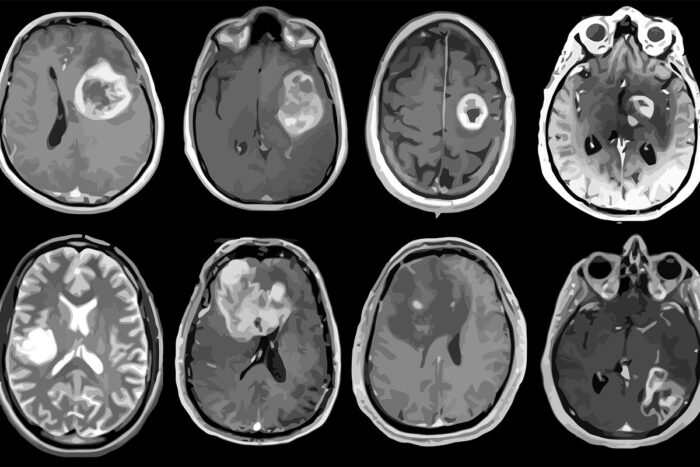
\includegraphics[height=1in]{brain-scans.jpg}
	\hfill	\pause
	\qquad 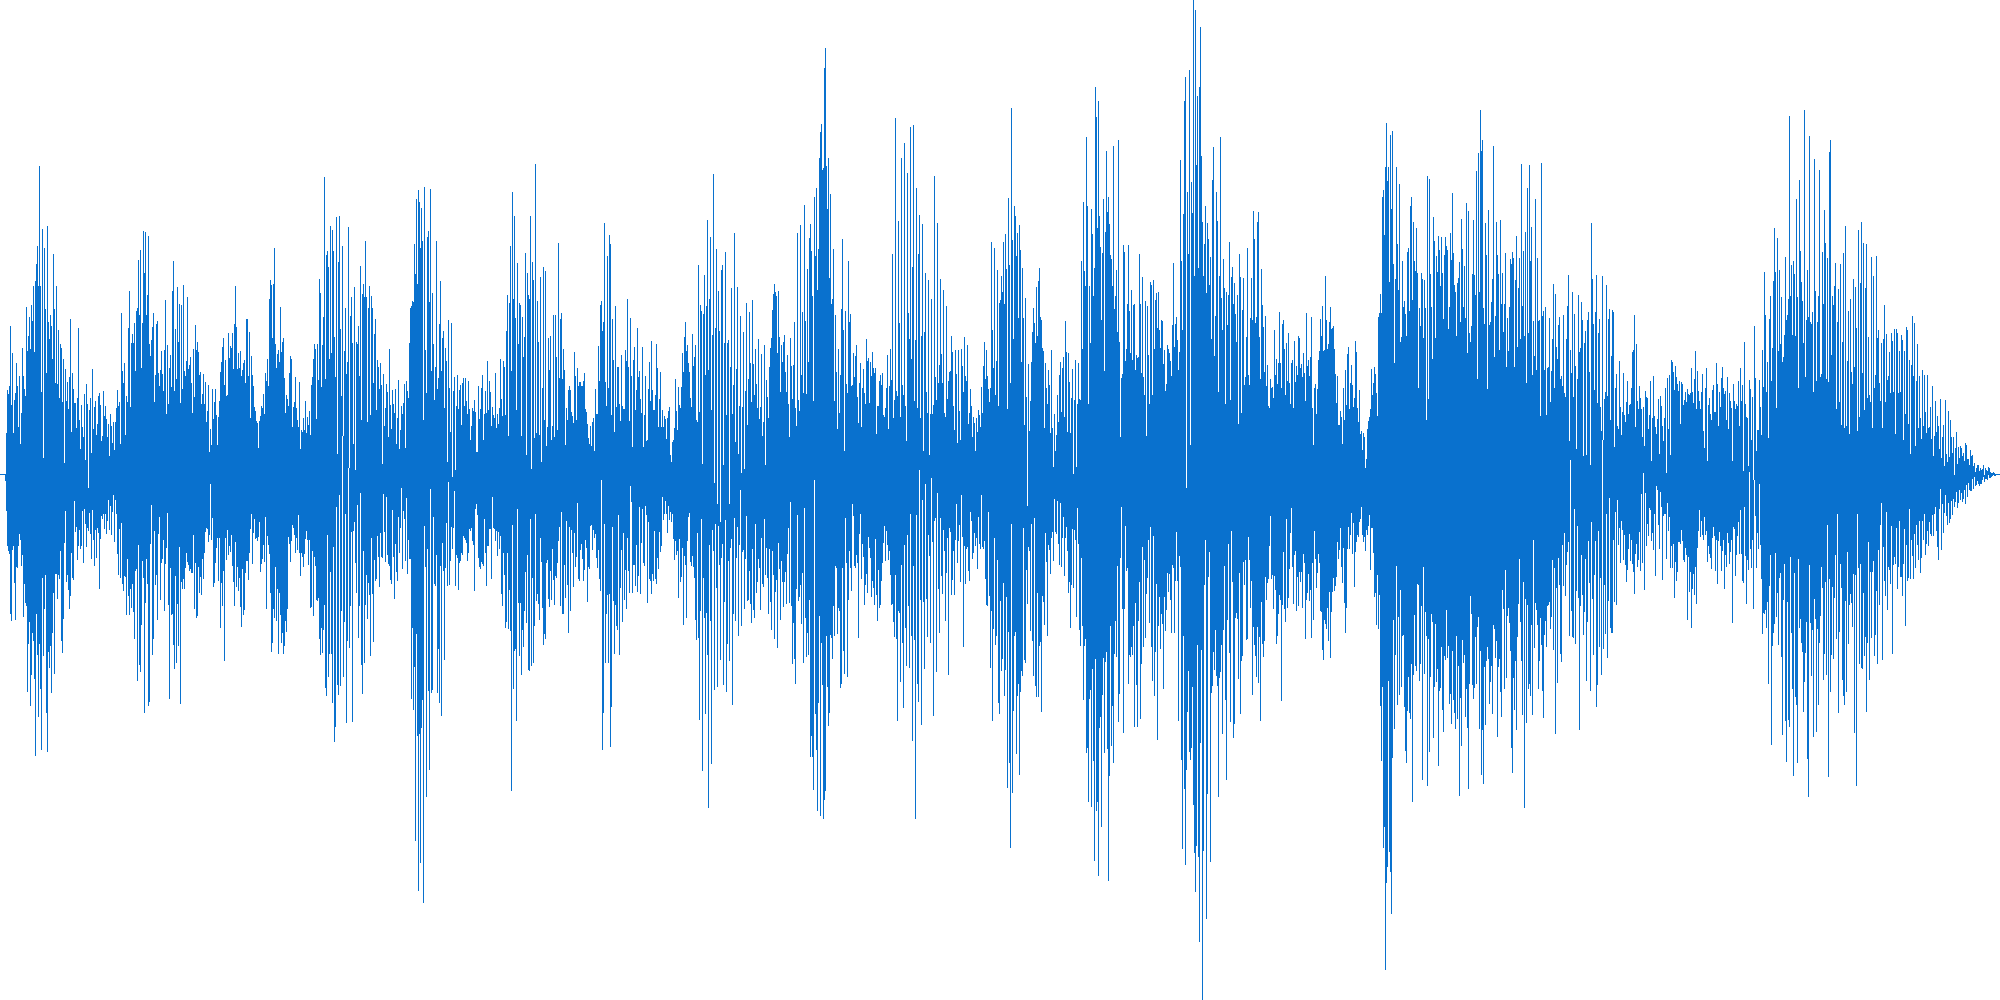
\includegraphics[height=1in]{audio-signal.png}

	\pause \bigskip

	\begin{center}
		% TODO: come up with something funnier here?
		\texttt{"Carleton College is in Northfield, Minnesota"}

		$\downarrow$

		$\langle 54, 138, 13, 40, 190, 72 \rangle$
	\end{center}

	\pause \bigskip

	\note{Okay, these things are very expressive and very powerful, but we're sweeping a huge amount under the rug.}

	\textbf{How do we estimate the parameters?}
\end{frame}

\begin{frame}{Training}

	Observations $x_i$, labels $y_i$, and a model $f_\beta(x_i)$.

	\pause \bigskip

	We want to find
	\begin{equation}
		\argmin_\beta \sum_i \ell(f(x_i), y_i)
	\end{equation}
	where $\ell$ is some "loss function".

	\pause \bigskip

	Ideas:

	\begin{enumerate}
		\item Least squares? ($\ell(a, b) = ||a - b||^2$)
		\item Maximum likelihood estimation?
	\end{enumerate}

\end{frame}

\begin{frame}{Gradient Descent}

	\begin{center}
		\bfseries
		Chalkboard!

		\begin{equation}
			\argmin_x f(x)
		\end{equation}

		\begin{align*}
			f & : \R \to \R   \\
			f & : \R^2 \to \R \\
			  & \quad \vdots  \\
			f & : \R^n \to \R
		\end{align*}
	\end{center}

\end{frame}

\begin{frame}[fragile]{Backpropogation}

	\textbf{Key observation:} gradients of neural networks are easily computable.

	\begin{equation*}
		\argmin_\beta \sum_i \ell(f(x), y)
	\end{equation*}

	\pause

	\begin{equation*}
		f(x) = C \sigma(Ax + b)
	\end{equation*}

	\bigskip \pause

	\textbf{Computational graph of $f$:}

	\begin{center}
		\begin{tikzpicture}[
				every edge quotes/.style = {below, font=\tiny}
			]
			\matrix [
			matrix of math nodes,
			column sep=2em,
			row sep=2em,
			nodes={anchor=center},
			] {
			& |(A)|A        & |(b)| b &              & |(C)| C       & |(y)| y    &         \\
			|(x)| x & |(t1)| \times & |(p)| + & |(s)| \sigma & |(t2)| \times & |(l)| \ell & |(L)| {\text{loss}} \\
			};

			\draw[->] (x) -- (t1);
			\draw[->] (t1) edge["$x_1$"] (p);
			\draw[->] (p) edge["$x_2$"] (s);
			\draw[->] (s) edge["$x_3$"] (t2);
			\draw[->] (t2) edge["$f(x)$"] (l);
			\draw[->] (l) -- (L);

			\draw[->] (A) -- (t1);
			\draw[->] (b) -- (p);
			\draw[->] (C) -- (t2);
			\draw[->] (y) -- (l);
		\end{tikzpicture}
	\end{center}

	\medskip \pause
	
	% TODO: include this or not"
	% \begin{equation*}
	% 	\frac{\partial \ell}{\partial C}
	% 	= \frac{\partial \ell}{\partial f} \frac{\partial f}{\partial C}
	% \end{equation*}

	% TODO: do another example on the board

	\note{By keeping track of intermediate states, we can compute the gradient of the loss with respect to the parameters, and then update the parameters to move them closer to their optimal (loss-minimizing) states.}

\end{frame}

\begin{frame}[t]{Computational aside}

	In practice, modern neural networks have much more complicated computational graphs

	\only<+>{
		\begin{center}
			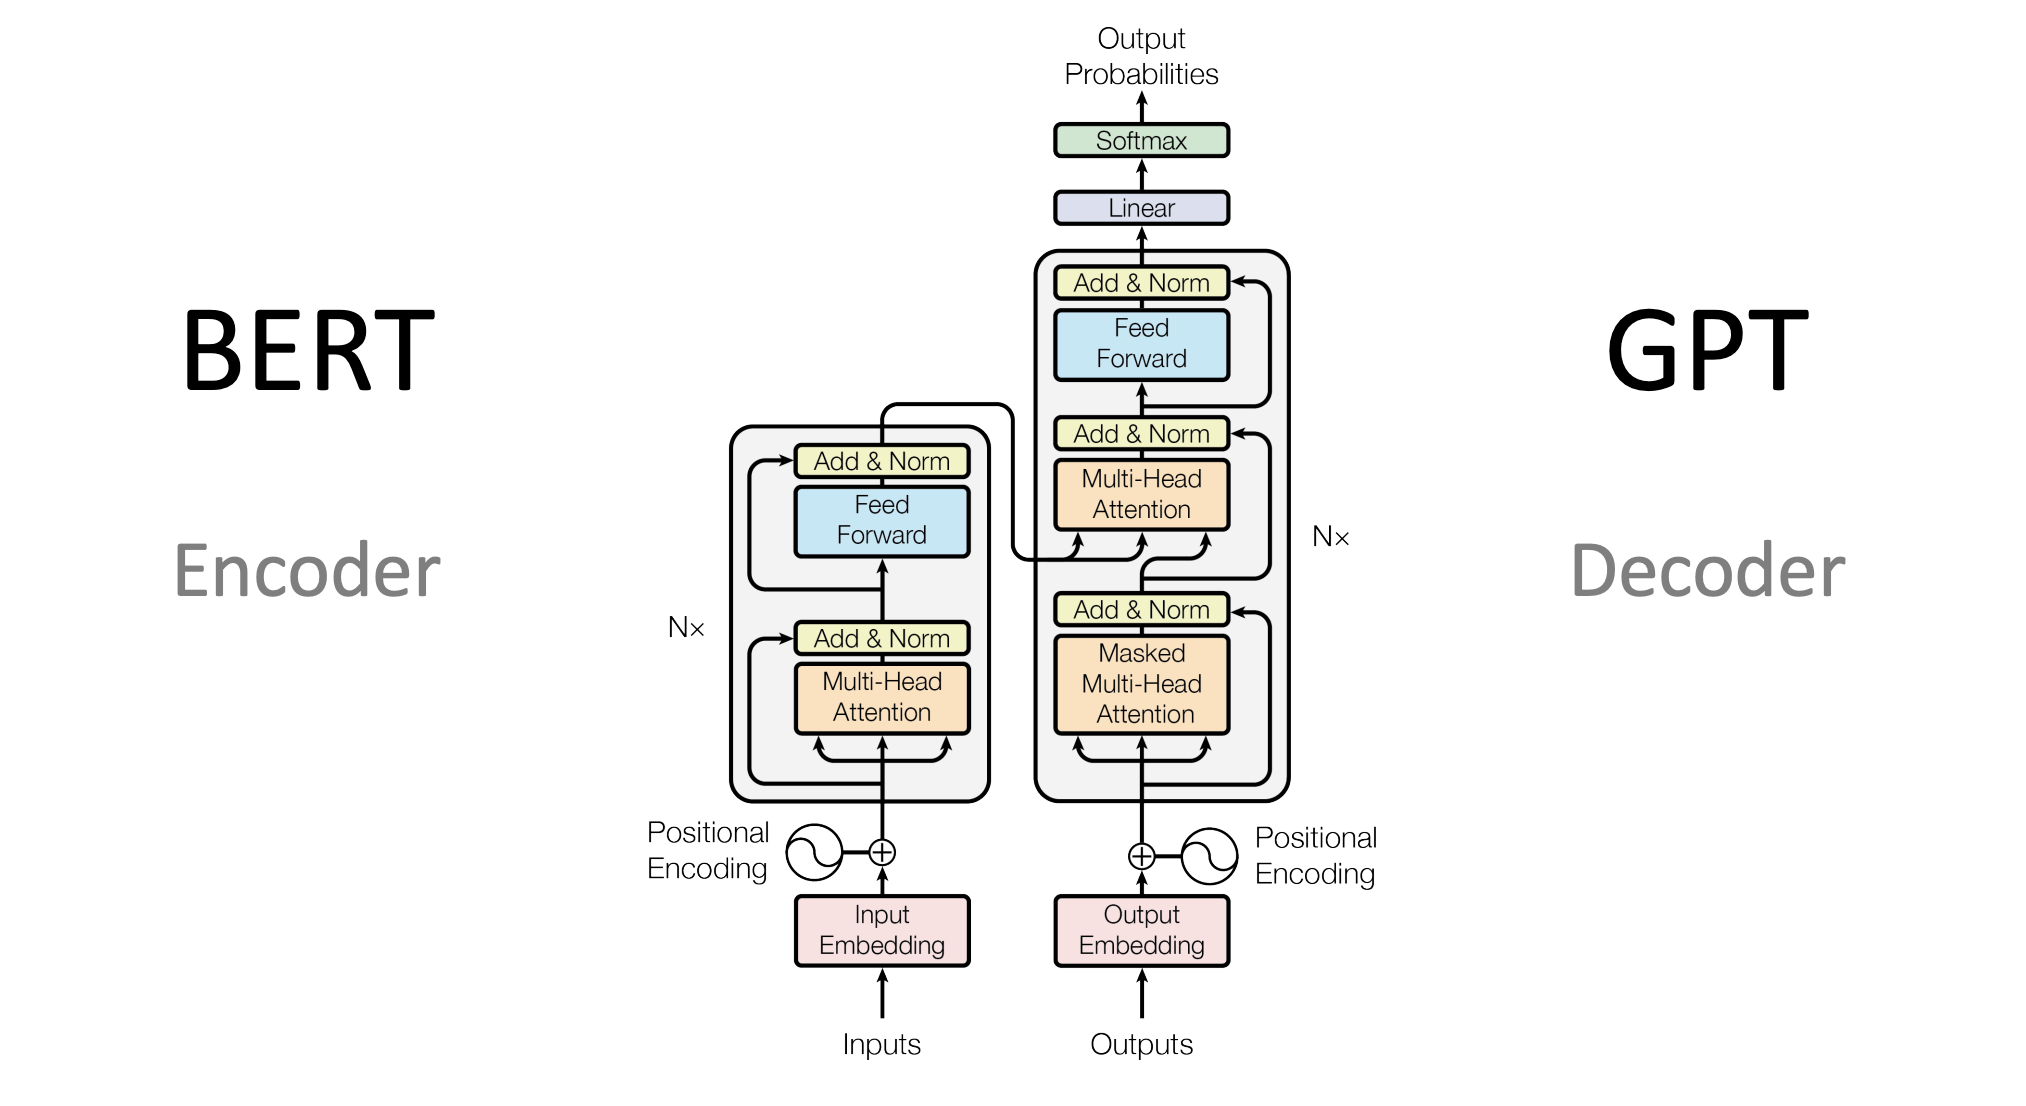
\includegraphics[width=\textwidth]{transfomer.png}
		\end{center}

		GPT 4 has $\sim 1$ trillion parameters ($\sim 4$ TB just to store them)
	}

	\pause \vspace{1in}

	Gradient descent scales surprisingly well, but...

	\pause \medskip

	...updating parameters (i.e. computing gradients) takes a \textit{lot} of compute.

	\note{Only recently that it's become computationally viable.}

	\note{People dedicate their lives to this sort of thing, this is just barely scratching the surface.}
\end{frame}

\begin{frame}[t]{Evaluation}

	\pause

	Is our model $\hat f_\beta$ a good approximation of the real process $f$?

	\note{Or "is appropriate"}

	\pause \bigskip

	\textbf{Familiar tools}

	\begin{itemize}[<+->]
		\item Goodness of fit
		\item Diagnostic plots
		\item AIC, BIC, etc.
	\end{itemize}

	\pause \bigskip

	\textbf{Cross-validation}

	``Give it some data it hasn't seen before and see how well it does.''

	\medskip \pause

	\begin{enumerate}
		\item Split your data into "training" and "test" subsets.
		\item Train your model on \emph{only} the training data.
		\item Evaluate your model's performance on the "test" data.
	\end{enumerate}
\end{frame}

\begin{frame}[t]{Evaluation}

	Is our model $\hat f_\beta$ a good approximation of the real process $f$?

	\begin{center}
		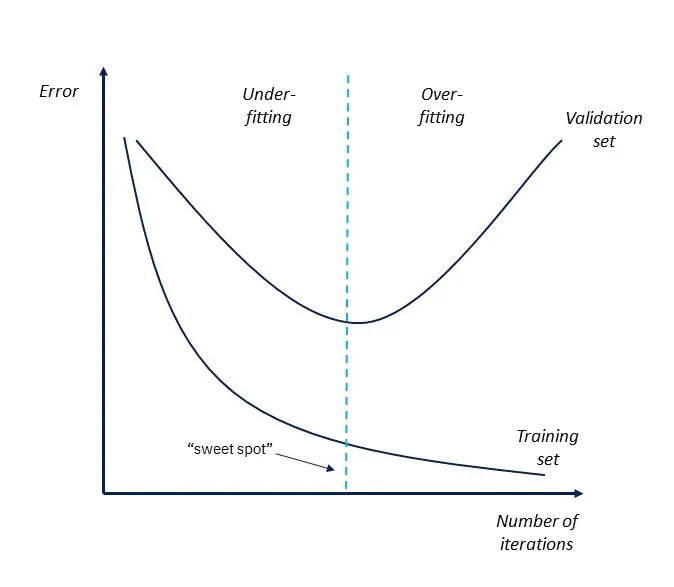
\includegraphics[width=.6\textwidth]{over-under-fitting.png}
	\end{center}

\end{frame}

\begin{frame}{Recap}
	\begin{itemize}
		\item Neural nets $=$ matrix multiplication + non-linearity.
		\item They can approximate pretty much any function.
		\item We train them with backpropagation and gradient descent.
		\item We estimate their performance with cross-validated loss.
	\end{itemize}
\end{frame}
